\documentclass[a4paper, 11pt, titlepage]{article}
\usepackage{fancyhdr}
\usepackage{graphicx}
\usepackage{imakeidx}
\usepackage{makeidx}
\usepackage{mathtools}
\usepackage[spanish]{babel}
\usepackage{eurosym}
\usepackage{hyperref}

% Variables
\newcommand{\nombre}{\emph{\textbf{El uso de pipelines en el procesador}}}

\title{\textbf{\nombre}\\ {\normalsize \textbf{Estructura de computadores}}}
\author{Francisco Javier Balón Aguilar}
\date{2020/2021}

% --------------------------------------------------------------------------------------------

\begin{document}
\maketitle
\renewcommand{\contentsname}{Índice}
\tableofcontents
\newpage

\section{Introducción}

    En computación, se le llama \textit{pipeline}, a la implementación de simultaneidad a nivel de instrucciones 
    dentro de un solo procesador, intentando mantener ocupada cada parte del procesador dividiendo las instrucciones 
    entrantes en una serie de pasos secuenciales, que se realizan por diferentes unidades del procesador que trabajan 
    de forma simultánea. De tal forma que aumenta el rendimiento de la CPU a una velocidad de reloj determinada, 
    aunque puede aumentar la latencia debido a la sobrecarga adicional del proceso de pipeline en sí. Pero esto lo veremos 
    más adelante en detalle.
    
    Es común hacer el símil con una cadena de montaje. Entender cómo funcionan los \textit{pipelines} es un paso 
    importante para entender cómo funcionan un procesador.

    El nombre, por analogía, viene de que para impulsar el gas en un oleoducto a la máxima velocidad posible es necesario 
    dividir el oleoducto en tramos y colocar una bomba que dé un nuevo impulso al gas. El símil con la programación existe 
    en que los cálculos deben ser registrados o sincronizados con el reloj cada cierto tiempo para que la ruta crítica 
    (tramo con más carga o retardo computacional entre dos registros de reloj) se reduzca. 

    El alto rendimiento y la velocidad elevada de los modernos microprocesadores, se debe, principalmente a la conjunción 
    de tres técnicas:

    \begin{itemize}
        \item La segmentación o pipelining.
        \item Arquitectura Harvard (arquitectura que propicia el paralelismo).
        \item Procesador de tipo RISC (véase sección \ref{risc}).
    \end{itemize}

\section{Historia}

    Como adelantamos en el apartado anterior, los pipelines funcionan de una forma similar a una cadena
    de montaje\footnote{
        De hecho, en términos anglosajones podemos equiparar pipelines a cadenas de montaje de cauce segmentado.
    }. No obstante, se aplicó por primera vez a principios del Siglo XX en la fabricación del 
    Ford T \footnote{
        \textit{<<The data flor through the computer [...] is comparable to a pipeline which, once filled, has a 
        large output rate no matter what its length.>>} Bucholtz, 1962.
    }

    Si atendemos al origen del uso de pipelines en computación, deberemos acudir a la \textit{IBM 704} (1955), 
    siendo ésta la máquina computadora mejora de la \textit{IBM 701}. Fue además la primera computadora producida 
    en masa con hardware basado en aritmética de coma flotante\footnote{
        La representación de punto flotante (en inglés floating point) es una forma de notación científica 
        usada en los computadores con la cual se pueden representar números reales extremadamente grandes y 
        pequeños de una manera muy eficiente y compacta, y con la que se pueden realizar operaciones 
        aritméticas.
    }. Precisamente esta aritmética contaba con un problema; 5 KFLOPS\footnote{
        FLOP (Operaciones de Coma Flotante por Segundo) es la unidad que mide el número de cálculos que puede 
        realizar una CPU (o GPU) por segundo. Un KFLOP corresponde a <<KiloFLOP>>, es decir, 1.000 FLOPS.
    }, provocando un cuello de botella en las operaciones I/O. Como solución a ello, incorporaron nuevos 
    procesadores I/O independientes (canales) en su sucesor, el \textit{IBM 709} (1958). Éste obtuvo de esta 
    forma una mejora del 60\% utilizando la misma frecuencia de reloj.

    Paralelamente, en 1956, nació el \textit{Proyecto Stretch}, con el objetivo de obtener una máquina 100 veces 
    más rápida que la \textit{IBM 704}. Para ello, era necesario que el procesador pudiese ejecutar simultáneamente 
    varias instrucciones. Para ello nació el \textit{IBM 7030}. Cabe destacar que no lograron su objetivo, ya 
    que en 1961 mediante benchmarks se demostró que únicamente lograron ser 30 veces más rápidos, y no 100, 
    debido a una alta latencia de recuperación de un error.
    
    En 1964, \textit{Seymour Cray} diseña y \textit{Control Data Corporation} produce el \textit{CDC 600}. 
    Éste fue el primer computador en utilizar múltiples unidades funcionales y procesadores periféricos (realmente 
    se trataban de 10 computadoras que dirigían los datos hacia una unidad central de proceso), logrando el hito 
    de superar en 3 la velocidad del Stretch, alcanzando 3 MIPs.

    A finales de la década de los 70s, el uso de pipelines paso a tener un papel de menor importancia, debido a 
    las tendencias de simplificación del software.

\section{Introducción a la ISA}

    Una ISA (Instruction Set Architecture) o arquitectura del conjunto de instrucciones es el repertorio de 
    instrucciones\footnote{
        Una instrucción no es más que un segmento de código que contiene implícita una operación que la CPU debe 
        realizar.
    } que puede entender y ejecutar la unidad de control de una determinada CPU. Eso no solo 
    incluye las instrucciones (tipos, codificación,…) comprensibles por la CPU, sino también el tipo de 
    datos aceptados de forma nativa, endianness, tamaño y cantidad de registros, arquitectura de la memoria, 
    e interrupciones/excepciones, extensiones, branching, etc. 

    En otras palabras, podríamos considerar a la ISA como la capa visible al programador a bajo nivel.

    Una ISA puede ser implementada (cómo se van a procesar o tratar sus instrucciones y datos) sobre lo que se 
    conoce como \textit{microarquitectura}\footnote{
        No hay que confundir el término microarquitectura ($\mu$arch) con arquitectura. Ésta segunda engloba 
        tanto la ISA como la microarquitectura, además de otros elementos y aspectos más amplios dentro del 
        sistema en conjunto del computador, que son estudiados en esta asignatura.
    }. Para ello será necesario contar con una serie de unidades funcionales
    (multiplexores, ALU, FPU, registros, unidad de control y demás circuitería).

    Diferentes microarquitecturas pueden ser compatibles con una misma ISA, pero una microarquitectura no 
    podrá procesar otra ISA diferente para la que fue diseñada; al menos de forma nativa.

\section{Tipos de ISA}

    Dentro de las ISAs encontramos varios tipos, que diferenciándolas \textit{grosso modo} en el tamaño 
    del repertorio de instrucciones y longitud obtenemos:

    \subsection{CISC}
    
        Son las siglas de Complex Instruction Set Computer, es decir, un modelo de 
        ISA complejo. Se compone de instrucciones largas, gran número de ellas y que pueden realizar 
        bastantes operaciones complejas con los oprandos situados en la memoria o registros. Aparecieron 
        antes que otros tipos, por eso CISC es un retrónimo. Algunos ejemplos de CISC son IBM System/370, 
        Zilog Z80, Motorola 68k, National Semiconductor 32016, MOS Technology 6502, DEC PDP-11, DEC VAX, 
        x86 (pre-x86, x86-8, x86-16, x86-32, x86-64), IBM z/Architecture, etc.

        Algunas características propias de este tipo son:

        \begin{itemize}
            \item La complejidad hace que el coste y el tiempo invertido en la implementación sea mayor.
            \item Suele tener una unidad de control microprogramada, más lenta y menos eficiente.
            \item Dispone de pocos bancos de registros de propósito general.
            \item Suelen ocupar más espacio en el silicio, lo que encarece su producción y baja el yield.
            \item Tamaño variable y largo. Gran cantidad de instrucciones, llegando a las 500 en algunos casos. 
            Necesitan varios ciclos de duración, por tanto el CPI es mayor, o lo que es lo mismo, el IPC es menor.
            \item Tenemos más cantidad de modos de direccionamiento y complejos.
            \item El tiempo de programación es menor, una de las pocas ventajas de CISC frente a RISC.
            \item El compilador no es crítico y puede ser más sencillo.
            \item El programa suele ser más compacto, ya que con pocas instrucciones complejas basta.
            \item La abstracción es alta, siendo el software algo más independiente del hardware.
        \end{itemize}

    \subsection{RISC}\label{risc}
    
        Son las siglas de Reduced Instruction Set Computer, es decir, un modelo de 
        ISA simple que surge para resolver algunos problemas destacados de los CISC. A finales de los 70 
        se comenzó a ver un fenómeno curioso, y es que algunas versiones de arquitecturas CISC de gama 
        baja a las que se le retiraban algunas de las instrucciones complejas para reducir costes en la 
        implementación, en vez de ir peor mejoraban su rendimiento. Por ese motivo se comienzan a diseñar 
        los primeros RISC con repertorios de instrucciones más reducidos e instrucciones simples. 
        Ejemplos son el AMD 29000, ARM, DEC Alpha, RISC-V, MIPS, HP PA-RISC, IBM PowerPC/POWER, SPARC, 
        etc.

        Algunas características propias de este tipo son:

        \begin{itemize}
            \item El tiempo de desarrollo para una microarquitectura de este tipo es más bajo y el coste más reducido.
            \item El tipo de unidad de control suele ser cableada, es decir, mucho más rápida y eficiente.
            \item Suelen tener gran cantidad de registros de propósito general.
            \item El espacio de integración es más bajo en igualdad de condiciones. Es decir, el dado o core tendrá 
            menor superficie.
            \item El tamaño de instrucciones es fija y corta. En cuanto a cantidad, suele ser reducido, normalmente 
            inferior a las 128 instrucciones. Suelen durar solo un ciclo de duración.
            \item La cantidad de modos de direccionamiento de memoria son pocos y simples.
            \item El tiempo de programación es más elevado.
            \item El compilador debe ser complejo y muy eficiente.
            \item El tamaño del programa generado es hasta un 30\% mayor al necesitar de más instrucciones 
            simples para realizar una misma tarea en comparación con CISC.
            \item La abstracción software/hardware es baja. El software está muy ligado al hardware.
        \end{itemize}

        \subsubsection{RISC-V}

            Dentro de las RISC existen muchas ISAs en actual uso, entre ellas las conocidas \textit{SuperH}, \textit{ARM} 
            (con buena relación rendimiento/eficiencia energética), \textit{RISC} y \textit{MIPS} (las primeras de ellas, por 
            ello llevan el nombre de RISC), etc.

            Pero la más moderna y que merece mención especial es \textit{RISC-V}. Ésta se desarrolla sobre una licencia 
            libre (\textit{BSD}). Iniciado por Berkeley con fondos del DARP, y actualmente participan en su creación multitud 
            de miembros de la fundación

    \subsection{Otros tipos}

        Aunque CISC y RISC son los dos grandes tipos de ISA y más relevantes, existen otros:
        
        \begin{itemize}
            \item \textbf{ZISC} Zero Instruction Set Computer no cuenta con un conjunto de instrucciones (en el sentido 
            clásico). Se basa en la mera coincidencia de patrones, similar a los computadores analógicos donde tampoco 
            existían, aunque aquí hablamos de computadoras digitales. Ha habido pocas implementaciones de este tipo, algún 
            ejemplo sería el IBM ZISC35 o el ZISC78, e incluso algunos chips neuronales como el CM1K…
            \item \textbf{SISC} Specific Instruction Set Computer es similar a RISC, de hecho se podría catalogar como tal, 
            pero es aún más reducidopara optimizar el rendimiento para alguna aplicación específica. Empleado en algunos 
            microcontroladores y ASIPs. Un ejemplo, algunos autores dicen que el DSP TMS320 de TI (Texas Instruments) es 
            SISC y otros lo etiquetan como RISC…
            \item \textbf{VISC} Virtual Instruction Set Computer es otro tipo introducido por Soft Machines.
            \item \textbf{DISC} Dynamic Instruction Set Computer puede modificar el conjunto de instrucciones de forma dinámica 
            según la demanda o exigencias del programa. Se suele usar para FPGAs reconfigurables.
            \item \textbf{NISC} No Instruction Set Computer tiene una tecnología muy específica de compilador y se emplea en 
            CPUs de alta eficiencia para algunas aplicaciones críticas, aceleradores por hardware, etc. No necesita de ROM de 
            microcódigo, ni controladores sofisticados, ni decodificador de instrucciones, etc.
            \item \textbf{MISC} Minimal Instruction Set Computer también es un conjunto muy reducido de instrucciones, pero a
            diferencia de otros como SISC o RISC, los operandos se almacenan en la pila en vez de en los registros, reduciendo 
            así el tamaño de los operandos y simplificando al máximo la microarquitectura. Funciona rápido y la unidad de 
            decodificación de instrucciones es más pequeña.
            \item \textbf{EDGE} Explicit Data Graph Execution intenta mejorar las carencias de CISC y evitar los problemas de 
            cuello de botella. Contiene muchas instrucciones individuales en un grupo denominado hyperblock y puede ser 
            ejecutado en paralelo.
            \item \textbf{OISC} One Instruction Set Computer, también llamado URISC (Ultimate RISC). Usa solo una instruccion 
            sin limitar las aplicaciones. Sus implementaciones se usan especialmente para la enseñanza. Imagina una instrucción 
            SUBLEQ que reste el contenido de dos direcciones de memoria y almacene el resultado en otra dirección. Con esa única 
            instrucción, ejecutandola secuencialmente se podrían conseguir los equivalentes a varias instrucciones. Por ejemplo, 
            si se ejecuta SUBLEQ b, b + SUBLEQ a, Z + SUBLEQ Z, b + SUBLEQ Z, Z = MOV a, b.            
        \end{itemize}

    \subsection{Híbridos CISC-RISC (RISC-Like)}

        Algunos diseñadores de microarquitecturas CISC han querido obtener las ventajas de RISC sin abandonar el modelo CISC o sin 
        perjudicar a la compatibilidad del software escrito para su ISA. Eso sería el caso de x86. CISC es un modelo antiguo y con 
        carencias, pero ¿cómo pasarse a RISC sin crear una nueva ISA y sin que todo el software compatible tenga que ser compilado 
        para esta nueva arqutiectura? La solución es la hibridación.

        Uno de los primeros diseños RISC-like sería el AMD K5, que usaba la exitosa microarquitectura del 29k a la que le añadieron 
        un Front-End para traducir las CISC-x86 y posibilitando que el Back-End trabajase de forma superescalar, con ejecución fuera 
        de orden, ejecución especulativa, renombre de registros, etc., sin alterar la compatibilidad con x86.

        Actualmente, los diseños de Intel y AMD trabajan como RISC a nivel electrónico, aunque el repertorio de instrucciones sea 
        CISC.

\section{Funcionalidad del procesador segmentado}

    Como hemos visto, utilizar pipelines o segmentar un procesador nos permite obtener una mayor agilidad y velocidad ejecutando varias 
    instrucciones al mismo tiempo (Se  comienza  la  próxima  instrucción mientras se trabaja aún en otra.). Las etapas son divididas 
    mediante registros, y en cada una de ellas puede estar ejecutándose una 
    instrucción (en 5 etapas pueden ejecutarse simultáneamente 5 instrucciones). Es  preciso, que cada instrucción pase por cada una 
    de las etapas, y que cada etapa tenga su propio control. 

    Basándonos en las etapas de instrucción del procesador \textit{DLX}\footnote{
        El DLX es un microprocesador RISC diseñado por John Hennessy y David A. Patterson, los diseñadores principales de la 
        arquitectura MIPS y de Berkeley RISC (respectivamente), los dos ejemplos de la arquitectura RISC. El DLX es básicamente 
        un MIPS revisado y simplificado con una arquitectura simple de carga/almacenamiento de 32 bits. Pensado principalmente 
        para propósitos educativos, se utiliza ampliamente en cursos de nivel universitario sobre arquitectura de computadores. 
    }, podemos dividir las etapas en las siguientes:

    \begin{itemize}
        \item Búsqueda de instrucción [BI] / Instruction fetch [IF].
        \item Decodificación, lectura de registros [Dec] / Instrucción decode [ID].
        \item Ejecución [Eje] / Execution [EX].
        \item Operación con memoria de datos [Mem] / Memory [MEM].
        \item Escritura en arreglo de registros [WR] / Writeback [WB].
    \end{itemize}

    \begin{figure}[htp]
        \centering
        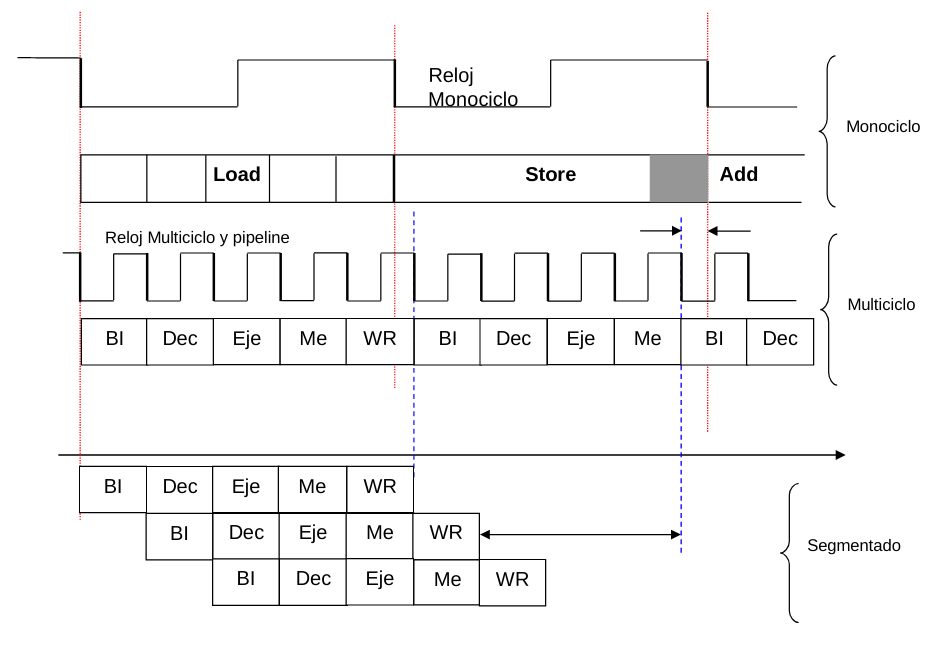
\includegraphics[width=1\textwidth]{resources/pipe00.png}
        \caption{Diferenciación gráfica de ejecuciones monoclico, multiciclo y segmentadas.}
        \label{pipe00}
    \end{figure}

    Como observamos en la figura \ref{pipe00}, atentiendo a la \textbf{ejecución monociclo}, el período del reloj lo establece la 
    instrucción que más tarda en ejecutarse, siendo éste la suma de los tiempos asociados a cada etapa.

    Los tiempos de acceso a memoria de instrucciones y de datos se asumen iguales y levemente mayores que la operación  
    de la Unidad Aritmético Lógica (ALU); la lectura y escritura de registros también se asumen iguales, y menores que el tiempo
    de propagación en la ALU.

    Si atendemos a la \textbf{ejecución multiciclo}, el período de reloj lo establece la etapa que más tarda en realizarse. Observamos 
    una mejora sustancial en la velocidad de ejecución en cada etapa. Pero cada ciclo de instrucciones empieza cuando termina el anterior.

    Finalmente, estudiamos el caso que nos atañe, siendo éste la \textbf{ejecución segmentada} --ó \textbf{pipeline}-- que, asumiendo 
    que cada instrucción ocupa todas las etapas, la realización individual de cada una de ellas está limitada por la etapa más lenta. 
    En la mayor parte del ciclo de reloj, el procesador se encuentra ejecutándo alguna etapa de todos los ciclos de instrucción habidos 
    en el ejemplo gráfico, finalizando todas las etapas prácticamente al mismo tiempo en que la ejecución multiciclo termina el primer 
    lote.

    \subsection{Riesgos del pipelining}

        Los riesgos de esta práctica en la mejora de procesos que podemos encontrar son:

        \subsubsection{Riesgos estructurales}

            Existen conflictos de hardware en distintas etapas de ejecución, ya que cada unidad funcional de memoria puede ser utilizada sólo 
            una vez por instrucción, así como cada unidad funcional debe ser usada en el mismo estado por todas las instrucciones.

            Como solución a ello, es necesario definir un estado de memoria que no hace nada.

        \subsubsection{Riesgos de control}

            Bloqueos después de cada salto por si hay que esperar la próxima instrucción.
            
            Predicción de saltos, ejecutando el salto de forma paralela con todas las instrucciones.

        \subsubsection{Riesgos de datos}

            Una instrucción depende del resultado previo, por lo que es necesario actualizar a tiempo el valor de las variables que van a ser 
            ocupadas.

        \subsubsection{Manejo de instrucciones}

            Las excepciones se pueden producir en los siguientes casos:

            \begin{itemize}
                \item Desbordamiento aritmético.
                \item Petición de I/O.
                \item Intento de uso de instrucciones privilegiadas.
                \item Mal funcionamiento de la circuitería.
            \end{itemize}

            La asociación de manera correcta de la excepción con la instrucción que la causó es problemático en los computadores segmentados.

\section{Pipelines en programación}

    La arquitectura en pipeline (basada en filtros) consiste en ir transformando un flujo de datos en un proceso comprendido por varias fases 
    secuenciales, siendo la entrada de cada una la salida de la anterior. 

    Esto aprovecha en el sistema operativo (o aplicaciones de alto nivel) las capacidades de los procesadores segmentados para permitir 
    al usuario ganar un mejor rendimiento y mayor velocidad en el desarrollo de los comandos. 

    Un ejemplo clásico son los pipelines en el entorno Unix y su familia (*nix Like). Especialmente nos centraremos en 
    el que se puede considerar como el heredero de Unix; GNU/Linux.

    Es necesario comprender primero los \textit{flujos de datos} en el entorno *nix (véase figura \ref{std00}):

    \begin{itemize}
        \item \textbf{STDIN (0)}. Entrada estándar, que representa la forma en que se ingresan datos al programa.
        \item \textbf{STDOUT (1)}. Salida estándar, que representa los datos que salen del programa (generalmente hace referencia a la pantalla).
        \item \textbf{STDERR (2)}. Salida de error estándar.
    \end{itemize}

    \begin{figure}[htp]
        \centering
        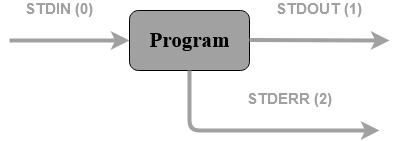
\includegraphics[width=0.5\textwidth]{resources/std00.png}
        \caption{Representación gráfica de flujos de datos.}
        \label{std00}
    \end{figure}

    Sin entrar en redirecciones de flujo, puesto que no es competencia de este trabajo, un pipeline o tubería consiste
    sencillamente en convertir la stdout de un programa en stdin de otro, encadenando las órdenes (véase figura \ref{pipe01}).

    \begin{figure}[htp]
        \centering
        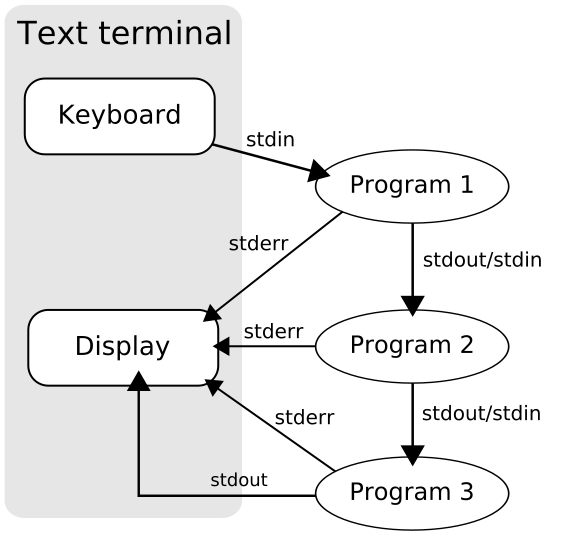
\includegraphics[width=0.5\textwidth]{resources/pipe01.png}
        \caption{Representación gráfica de pipelines en entorno Unix.}
        \label{pipe01}
    \end{figure}

    Para su muestra y prueba de concepto, observamos en la figura \ref{pipe02} el uso de dos pipelines para encadenar 3 comandos.

    \begin{figure}[htp]
        \centering
        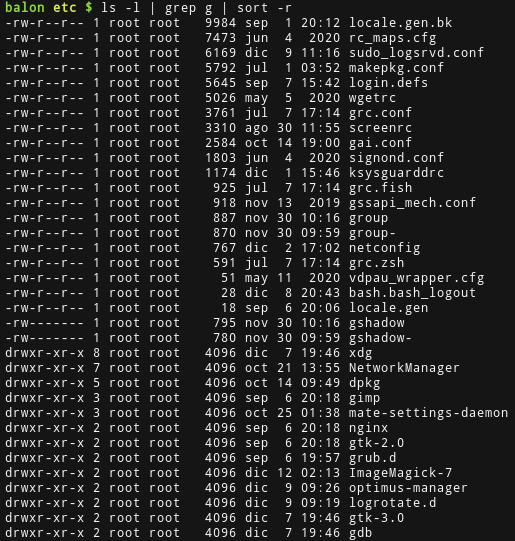
\includegraphics[width=0.7\textwidth]{resources/pipe02.png}
        \caption{Prueba de concepto con tuberías en GNU/Linux.}
        \label{pipe02}
    \end{figure}


% BIBLIOGRAFÍA Y REFERENCIAS
\newpage
\begin{thebibliography}{X}
    \bibitem{} Data Pipeline Development (English) Publicado por Dativa, recuperado el 24 de mayo de 2018 \\ \url{https://deductive.com/data-pipelines/}
    \bibitem{} Historia del "Pipieline", Juan Antonio Romano Largo \\ \url{http://www.dacya.ucm.es/hidalgo/arquitectura/pipeline.pdf}
    \bibitem{} Introducción a la ISA, Architecnología \\ \url{https://architecnologia.es/risc-v-introduccion-a-la-isa}
    \bibitem{} RISC-V: similitudes y diferencias con otras ISAs tipo RISC, Architecnología \\ \footnotesize \url{https://architecnologia.es/risc-v-similitudes-y-diferencias-con-otras-isas-tipo-risc}
    \bibitem{} Segmentación y procesadores segmentados, ARCO - UPC \\ \url{https://studies.ac.upc.edu/EUPVG/ARCO_I/tema2.pdf}
    \bibitem{} Procesador Segmentado, Tomás V. Arredondo \\ \url{http://profesores.elo.utfsm.cl/~tarredondo/info/comp-architecture/paralelo2/C12_Diseno_Procesador_Segmentado.pdf}
    \bibitem{} The DLX Processor \\ \url{https://www.csee.umbc.edu/courses/undergraduate/411/spring96/dlx.html}
    \bibitem{} DLX Instructions \\ \url{https://www.eng.tau.ac.il/~guy/Computer_Structure03/slides/instructions.pdf}
    \bibitem{} Advanced UNIX Programming (Second Edition) Marc J. Rochkind (English)
    \bibitem{} LPIC-1 103-4 Flujos, tuberías y redirecciones, Architecnología \\ \url{https://architecnologia.es/lpic-1-tema-103-4-flujos-tuberias-redirecciones}
\end{thebibliography}

\end{document}